\section{Технический проект}
\subsection{Общая характеристика организации решения задачи}

Задача заключается в разработке и программной реализации веб-приложения для управления проектами, основанного на использовании Kanban-доски и принципов Agile-методологий. Приложение предназначено для командной работы и поможет руководителям проектов, а также членам команд эффективно планировать спринты и текущую деятельность, визуализировать рабочие процессы, отслеживать выполнение задач и улучшать взаимодействие, что способствует повышению общей продуктивности и успешности проектов.

Приложение будет представлять собой многопользовательское веб-приложение, доступное через сеть Интернет. Основными элементами интерфейса будут являться интерактивная Kanban-доска для визуального управления задачами, страницы для настройки проектов и досок, а также инструменты для работы с задачами.

\subsection{Обоснование выбора технологии проектирования}

Для создания приложения выбраны технологии, которые обеспечивают высокую производительность и удобство для пользователей. 

\subsubsection{Язык программирования JavaScript}
JavaScript — это высокоуровневый, мультипарадигменный язык программирования, являющийся ключевой технологией для создания интерактивных веб-сайтов и приложений. Он выполняется непосредственно в браузере пользователя, обеспечивая динамическое обновление контента и взаимодействие без перезагрузки страницы, а также может использоваться на серверной стороне благодаря среде Node.js \cite{javascript1}.

\subsubsection{Среда выполнения Node.js}
Node.js — это кроссплатформенная среда выполнения JavaScript, построенная на движке V8 от Google Chrome. Она позволяет исполнять JavaScript-код на стороне сервера, что открывает возможности для создания быстрых и масштабируемых сетевых приложений \cite{nodejs1}.

\subsubsection{Библиотека React}
React — это популярная JavaScript-библиотека для создания пользовательских интерфейсов, разработанная и поддерживаемая Facebook (ныне Meta). В основе React лежит концепция компонентного подхода, позволяющая разбивать сложный интерфейс на независимые, переиспользуемые части — компоненты, каждый из которых управляет собственным состоянием \cite{react1}.

\subsubsection{PostgreSQL}

PostgreSQL — это объектно-реляционная система управления базами данных, известная своей надежностью, гибкостью и расширяемостью. Она поддерживает широкий спектр функциональности, включая сложные запросы, транзакции, уровни изоляции и возможность создания пользовательских типов данных \cite{postgres1}.

\subsection{Диаграмма компонентов}

 На рисунке \ref{components_diagram.eps:image} изображена диаграмма компонентов системы.
 
 \begin{figure}[ht]
 	\center{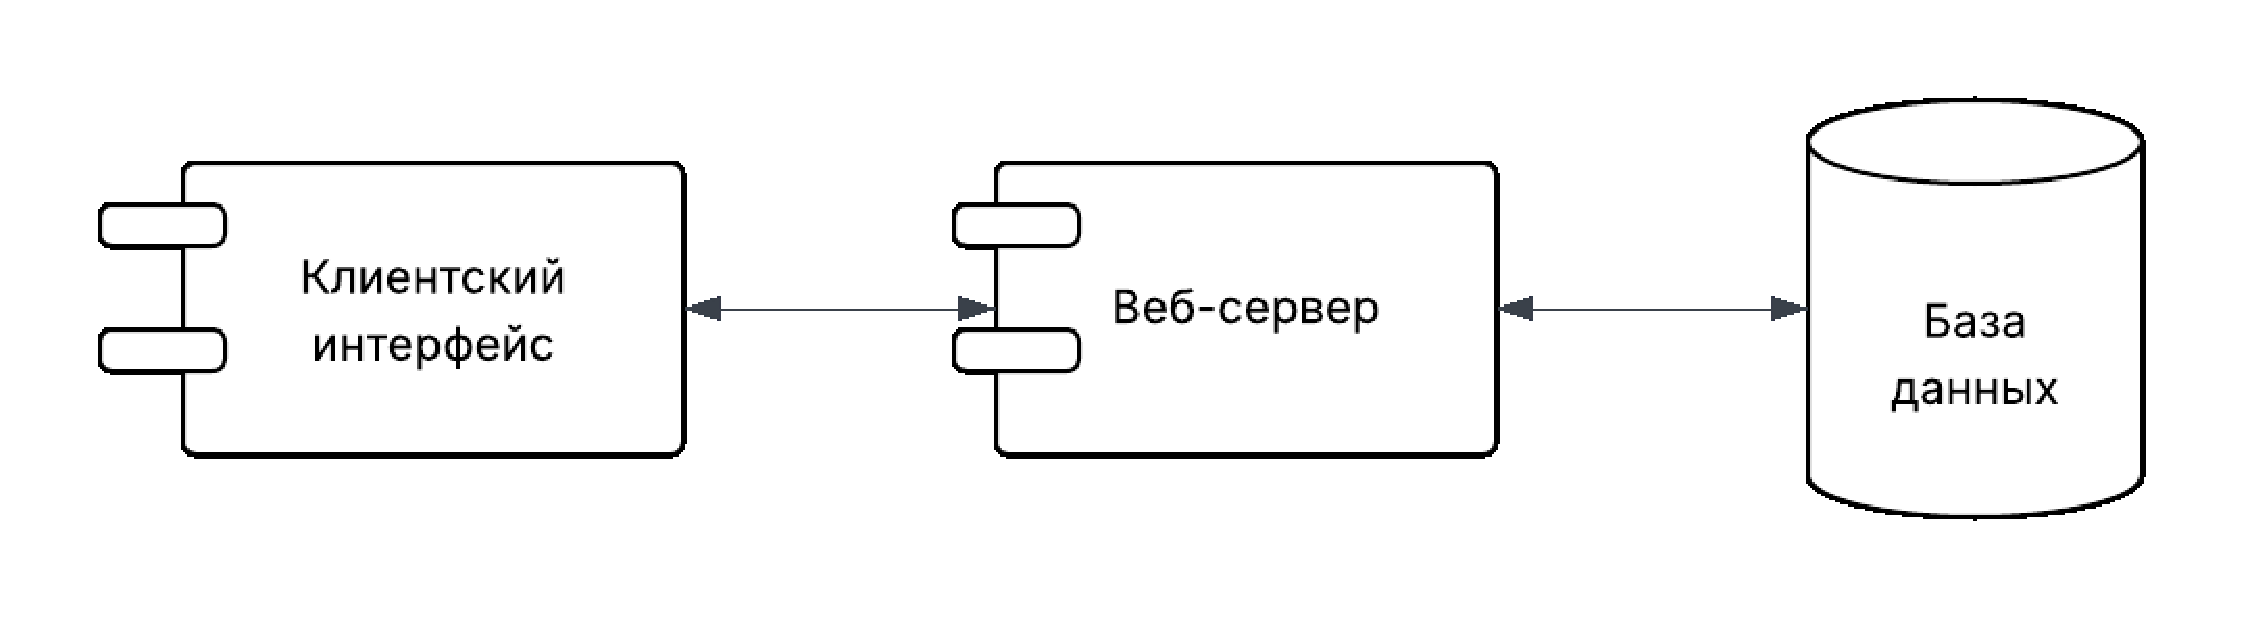
\includegraphics[width=1\linewidth]{components_diagram}}
 	\caption{Диаграмма компонентов}
 	\label{components_diagram.eps:image}
 \end{figure}
 
 На представленной диаграмме показана архитектура веб-приложения для управления проектами, основанного на Kanban-доске и Agile-методиках. Схема включает три основных компонента: «Клиентский интерфейс», «Веб-сервер» и «База данных». Эти компоненты соединены стрелками, которые указывают направление потоков данных и взаимодействия между ними. Каждая часть системы выполняет свои специфические функции, обеспечивая совместную и эффективную работу всего приложения.
 
 «Клиентский интерфейс» — это веб-приложение, которое запускается в браузере пользователя и служит основной точкой взаимодействия с системой. Через него пользователи могут регистрироваться и аутентифицироваться, создавать новые проекты, настраивать Kanban-доски, добавлять, редактировать и перемещать задачи между колонками. На страницах интерфейса в реальном времени отображается актуальное состояние проектов, Kanban-доски, списки задач, бэклоги и другая информация, необходимая для организации работы по Agile-принципам.
 
 «Веб-сервер» функционирует как центральный узел архитектуры, обрабатывающий всю бизнес-логику системы. Он получает HTTP-запросы от «Клиентского интерфейса», выполняет соответствующие операции, взаимодействует с «Базой данных» для сохранения или извлечения необходимой информации, и отправляет ответы «Клиентскому интерфейсу» для обновления отображаемых данных или подтверждения выполненных действий.
 
 «База данных» отвечает за надежное и долговременное хранение всей информации, используемой в системе управления проектами. В ней содержатся структурированные данные о зарегистрированных пользователях, созданных проектах, деталях задач, конфигурациях Kanban-досок и другие сведения, необходимые для функционирования Agile-процессов. «Веб-сервер» постоянно обращается к «Базе данных» для выполнения операций чтения и записи данных при каждом значимом взаимодействии пользователя с системой.
 
\subsection{Структура программы}
Система управления проектами представляет собой веб-приложение, чья структура организована в виде набора модулей, каждый из которых выполняет определённые функции.
\subsubsection{Клиентская часть}
Клиентская часть приложения разработана с использованием библиотеки React и отвечает за пользовательский интерфейс и взаимодействие с пользователем. Она включает в себя набор компонентов, каждый из которых выполняет определенную функцию, начиная от отображения основных элементов управления и заканчивая сложными модальными окнами для управления данными:
\begin{enumerate}
	\item Модуль App.jsx. Главный компонент React-приложения. Управляет состоянием аутентификации пользователя, маршрутизацией между основными представлениями, отображением глобальных модальных окон. Инициализирует загрузку основных данных при входе пользователя и при их обновлении.
	\item Модуль layoutObject.jsx. Компонент, определяющий основной макет интерфейса для аутентифицированных пользователей. Включает боковую панель настроек, верхнюю панель со списком проектов и поиском, а также основную область контента, где динамически отображаются либо доски Kanban с задачами, либо страница детального просмотра задачи. Реализует логику перетаскивания для досок и задач.
	\item Модуль authPage.jsx. Компонент страницы аутентификации. Предоставляет пользователю интерфейс для регистрации новой учетной записи и входа в существующую. Включает валидацию вводимых данных и отображение требований к паролю.
	\item Модуль userProfilePage.jsx. Компонент страницы профиля пользователя. Отображает информацию о текущем аутентифицированном пользователе и предоставляет функционал для редактирования и удаления профиля через соответствующие модальные окна.
	\item Модуль taskPage.jsx. Компонент страницы детального просмотра задачи. Отображает всю информацию о выбранной задаче, включая ее заголовок, описание, проект, доску, срок выполнения, приоритет, тип, автора, а также назначенных разработчика и QA-специалиста. Предоставляет пользователю возможность назначить себя на роль разработчика или QA, если эти роли свободны. Также содержит кнопки для редактирования и удаления задачи.
	\item Модуль boardObject.jsx. Компонент, представляющий одну доску Kanban в рамках проекта. Отображает заголовок и описание доски. Содержит список задач, принадлежащих этой доске, и обеспечивает возможность перетаскивания задач. Предоставляет кнопку для редактирования/удаления доски.
	\item Модуль taskObject.jsx. Компонент, представляющий карточку отдельной задачи на доске. Отображает заголовок задачи, ее тип, приоритет, срок выполнения, а также краткую информацию об авторе, разработчике и QA-специалисте. Позволяет пользователю кликнуть по карточке для перехода на страницу детального просмотра задачи.
	\item Модуль settingsPanel.jsx. Компонент боковой панели навигации и действий. Содержит кнопки для добавления новой задачи, перехода к профилю пользователя, добавления нового проекта, добавления новой доски, редактирования текущего проекта, управления участниками текущего проекта и выхода из системы. Видимость некоторых кнопок зависит от роли пользователя и выбранного проекта.
	\item Модуль projectsPanel.jsx. Компонент, отображаемый в верхней части интерфейса. Содержит выпадающий список для выбора текущего проекта из числа тех, в которых пользователь состоит.
	\item Модуль tooltipObject.jsx. Вспомогательный компонент для отображения всплывающих текстовых подсказок при наведении курсора на элементы интерфейса.
	\item Модуль modalObject.jsx. Компонент модального окна для создания новой задачи. Позволяет выбрать доску, ввести заголовок, описание, срок выполнения, а также выбрать приоритет и тип задачи.
	\item Модуль addBoardModal.jsx. Компонент модального окна для добавления новой доски в выбранный проект. Позволяет ввести заголовок и описание доски.
	\item Модуль addProjectModal.jsx. Компонент модального окна для создания нового проекта. Позволяет ввести название и описание проекта.
	\item Модуль alertModal.jsx. Общий компонент для отображения простых информационных сообщений или оповещений об ошибках с одной кнопкой «OK».
	\item Модуль confirmModal.jsx. Общий компонент для запроса подтверждения у пользователя перед выполнением деструктивных или важных действий. Предоставляет кнопки «Подтвердить» и «Отмена».
	\item Модуль editBoardModal.jsx. Компонент модального окна для редактирования существующей доски. Позволяет изменить заголовок и описание доски, а также удалить доску.
	\item Модуль editProfileModal.jsx. Компонент модального окна для редактирования персональной информации пользователя.
	\item Модуль editProjectModal.jsx. Компонент модального окна для редактирования существующего проекта. Позволяет изменить название и описание проекта, а также удалить проект.
	\item Модуль editTaskModal.jsx. Компонент модального окна для редактирования существующей задачи. Позволяет изменить заголовок, описание, доску и приоритет задачи.
	\item Модуль manageMembersModal.jsx. Компонент модального окна для управления участниками выбранного проекта. Позволяет просматривать список участников, добавлять новых участников по email и удалять существующих.
\end{enumerate}

\subsubsection{Серверная часть}
Серверная часть приложения, построенная на Node.js с использованием фреймворка Express.js, обеспечивает обработку всех API-запросов, управление бизнес-логикой, взаимодействие с базой данных и реализацию механизмов безопасности, таких как аутентификация и авторизация. Список связанных модулей:
\begin{enumerate}
	\item Модуль server.cjs. Основной файл серверной части приложения, реализованный на Node.js с использованием фреймворка Express.js. Отвечает за обработку всех API-запросов от клиентской части. Реализует эндпоинты для:
	\begin{itemize}
		\item регистрации и аутентификации пользователей;
		\item управления профилями пользователей;
		\item получения списка всех пользователей системы;
		\item управления проектами;
		\item управления участниками проектов;
		\item управления досками;
		\item управления задачами.
	\end{itemize}

Взаимодействует с базой данных PostgreSQL для хранения и извлечения данных. Реализует логику авторизации, проверяя права пользователя (например, владелец проекта, администратор, участник проекта) перед выполнением защищенных операций.
\end{enumerate}

\subsubsection{Клиентские сервисы}
Клиентские сервисы представляют собой вспомогательные JavaScript-модули, которые инкапсулируют специфическую логику, используемую различными компонентами клиентской части. Они помогают упростить взаимодействие с API и управление состоянием аутентификации. Список связанных модулей:
\begin{enumerate}
	\item Модуль apiService.js. Модуль на стороне клиента, предоставляющий функцию authenticatedFetch для упрощения выполнения аутентифицированных HTTP-запросов к API серверной части. Автоматически добавляет JWT токен аутентификации в заголовки запросов. Содержит логику для обработки специфических ошибок от сервера и вызова глобального обработчика для принудительного выхода пользователя из системы при проблемах с сессией или токеном.
	\item Модуль tokenService.js. Модуль на стороне клиента, предоставляющий утилиты для работы с JWT токеном. Включает функцию isTokenActive для проверки наличия токена в localStorage и валидации его срока действия путем декодирования с использованием jwt-decode.
\end{enumerate}
               
\subsubsection{Управление состоянием и стилизация}
Для эффективного управления состоянием приложения на стороне клиента используется библиотека Zustand, обеспечивающая централизованное и реактивное хранилище данных. Визуальное оформление реализуется с помощью Tailwind CSS и кастомных CSS-правил для создания консистентного и адаптивного пользовательского интерфейса. Список связанных модулей:
\begin{enumerate}
	\item Модуль store.js. Файл, определяющий глобальное хранилище состояния приложения с использованием библиотеки Zustand. Содержит состояние для проектов, досок, задач, информации о текущем пользователе, списке всех пользователей, текущем выбранном проекте и задаче, виде отображения приложения, а также различные флаги для модальных окон и оповещений. Реализует действия для изменения этого состояния. Использует middleware persist для сохранения части состояния в localStorage браузера.
	\item index.css. Основной файл стилей приложения. Включает базовые стили и утилиты Tailwind CSS, а также кастомные CSS-правила для оформления полос прокрутки и других элементов интерфейса для обеспечения единого визуального стиля.
\end{enumerate}

\subsubsection{Точка входа и конфигурация БД}
Этот раздел описывает основные файлы, отвечающие за запуск клиентского приложения, а также скрипт для инициализации и настройки структуры базы данных PostgreSQL, включая создание таблиц и заполнение начальными данными. Список связанных элементов:
\begin{enumerate}
	\item Модуль main.jsx. Точка входа клиентского React-приложения. Инициализирует корневой компонент App и рендерит его в DOM-элемент с id root. Подключает основные стили из index.css.
	\item db.sql. SQL-скрипт, предназначенный для инициализации структуры базы данных PostgreSQL. Содержит команды создания для всех необходимых сущностей, определяет первичные и внешние ключи, ограничения, значения по умолчанию и триггеры для автоматического обновления временных меток. Также включает секцию для заполнения базы данных начальными тестовыми данными для демонстрации и тестирования функционала.
\end{enumerate}

Структура и отношения между модулями представлены на диаграмме модулей.
 \begin{figure}[ht]
	\center{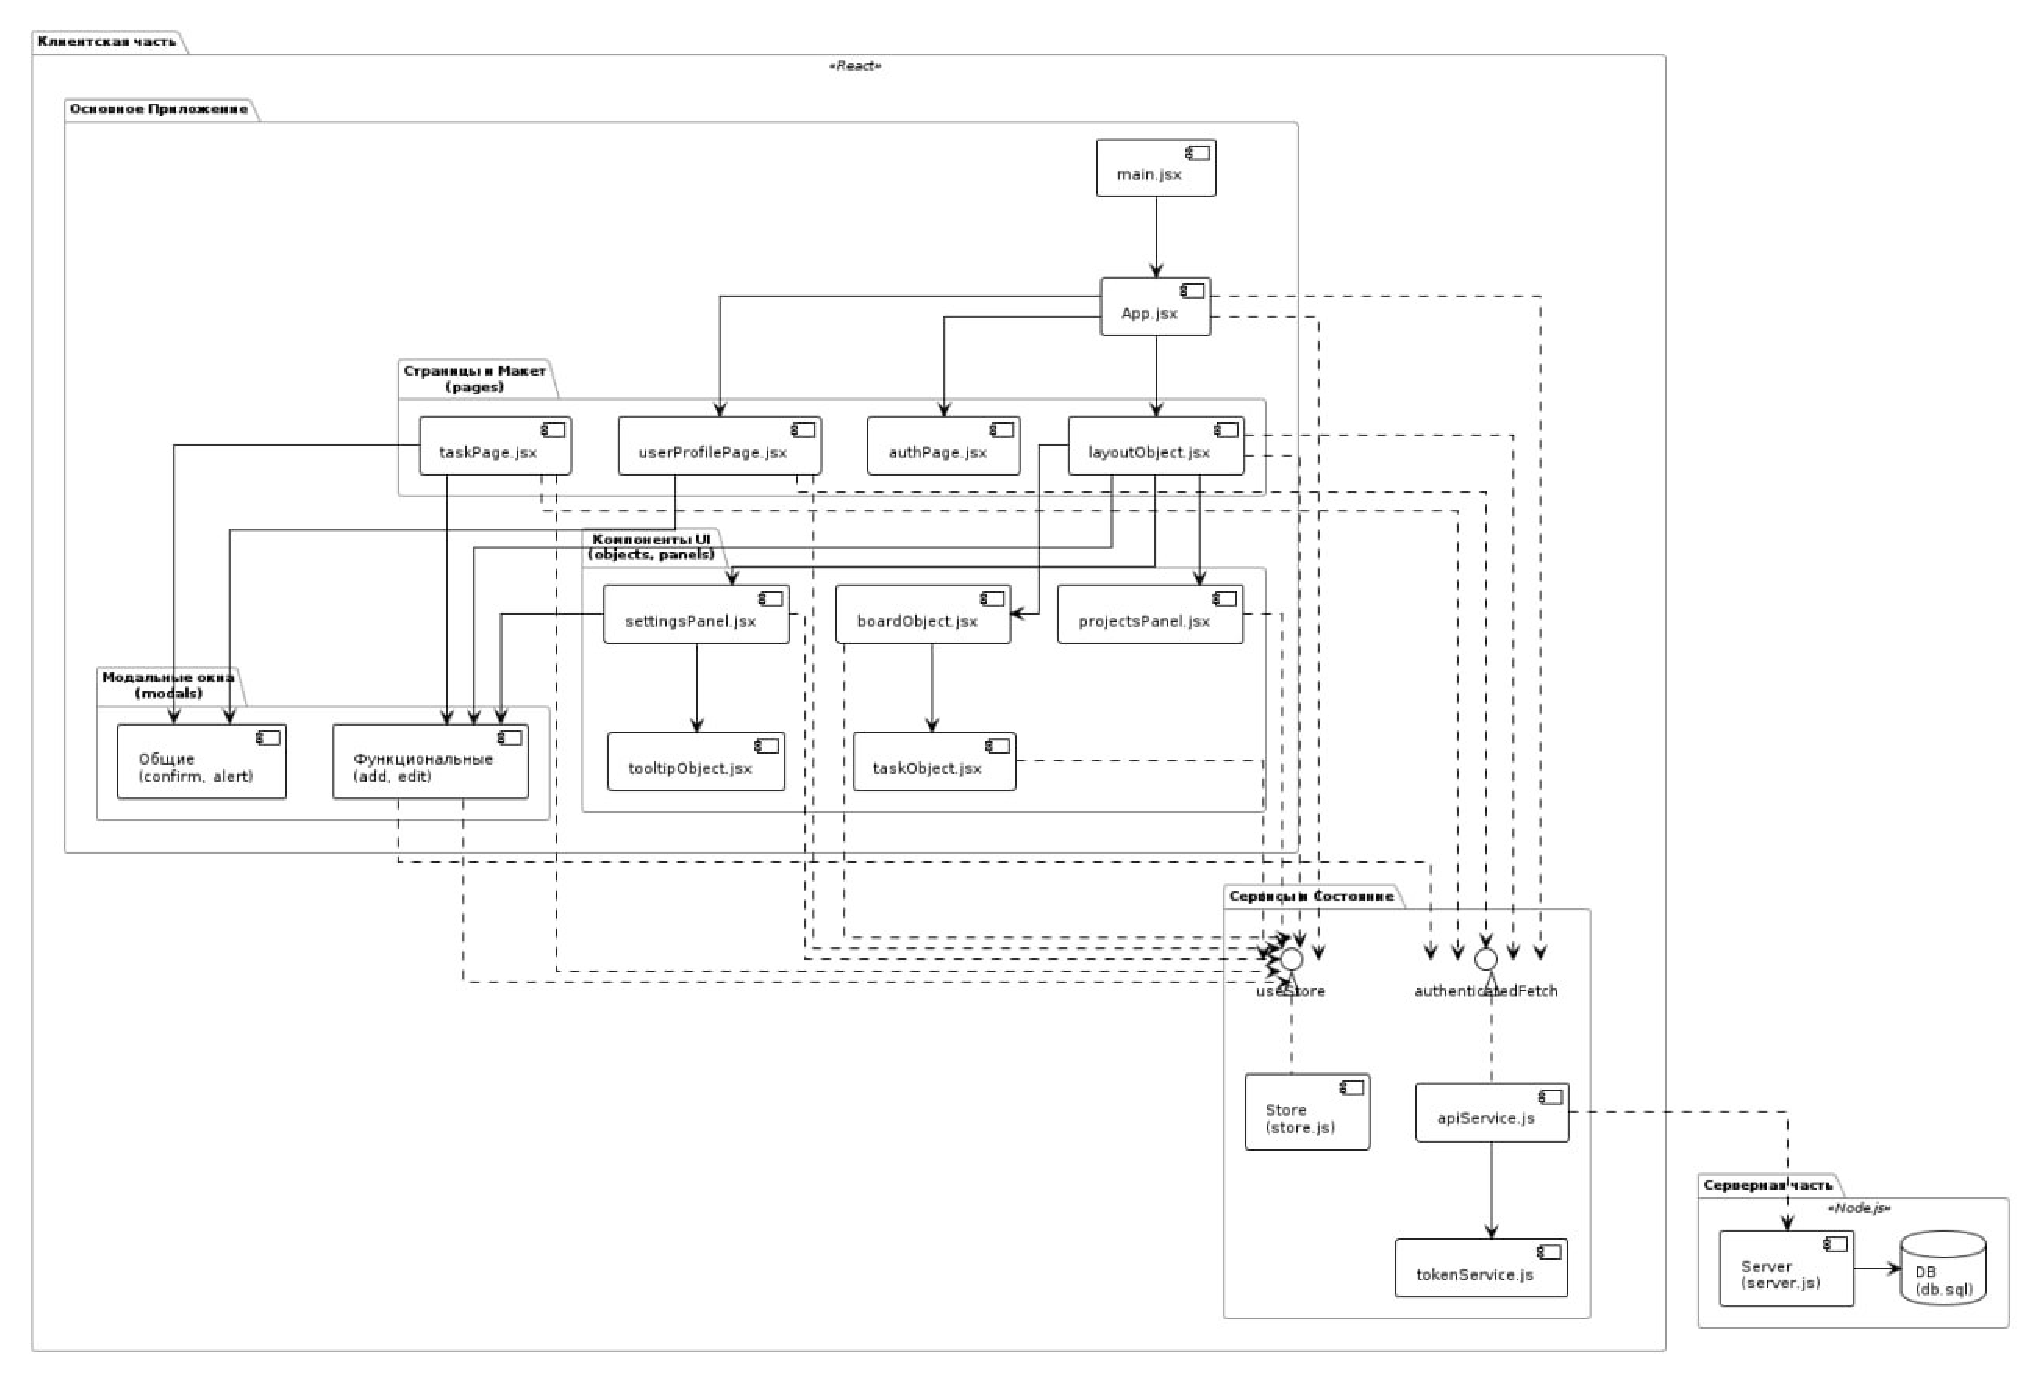
\includegraphics[width=1\linewidth]{modules_diagram}}
	\caption{Диаграмма модулей}
	\label{modules_diagram:image}
\end{figure}

\subsection{Структура базы данных}
Сущности и отношения между ними отображены на ER-диаграмме.
 \begin{figure}[ht]
	\center{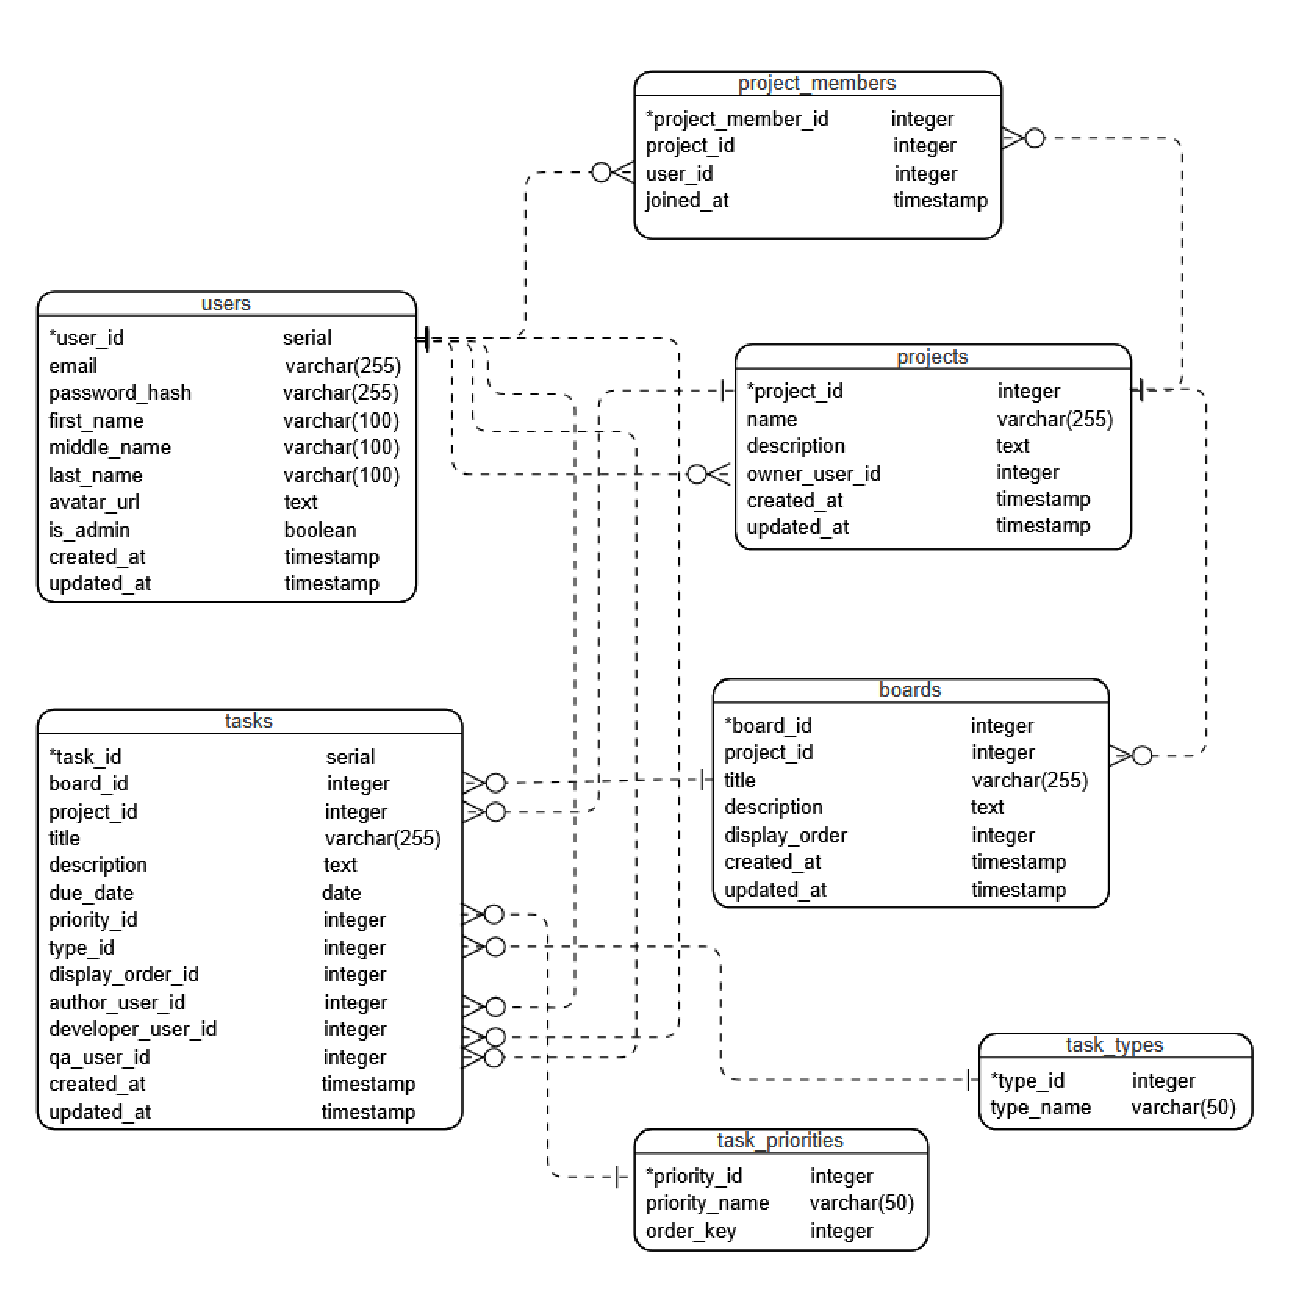
\includegraphics[width=1\linewidth]{er_diagram}}
	\caption{ER-диаграмма}
	\label{er_diagram:image}
\end{figure}
\begin{xltabular}{\textwidth}{|p{2.5cm}|p{4cm}|p{1.7cm}|X|}
	\caption{Атрибуты сущности «Users»\label{users:table}}\\ \hline
	\centrow Поле & \centrow Тип & \centrow Обяза\-тельное & \centrow Описание \\ \hline
	\thead{1} & \thead{2} & \centrow 3 & \centrow 4 \\ \hline
	\endfirsthead
	\caption*{Продолжение таблицы \ref{users:table}} \\ \hline
	\thead{1} & \thead{2} & \centrow 3 & \centrow 4 \\ \hline
	\finishhead
	user\_id & serial & \centrow да & Первичный ключ, уникальный идентификатор пользователя. \\ \hline
	email & varchar(255) & \centrow да & Адрес электронной почты пользователя, уникальный. \\ \hline
	password\_ hash & varchar(255) & \centrow да & Хеш пароля пользователя. \\ \hline
	first\_name & varchar(100) & \centrow нет & Имя пользователя. \\ \hline
	middle\_ name & varchar(100) & \centrow нет & Отчество пользователя. \\ \hline
	last\_name & varchar(100) & \centrow нет & Фамилия пользователя. \\ \hline
	avatar\_url & text & \centrow нет & URL-адрес аватара пользователя. \\ \hline
	is\_admin & boolean & \centrow да & Флаг, указывающий, является ли пользователь администратором. \\ \hline
	created\_at & timestamp with time zone & \centrow да & Дата и время создания записи. \\ \hline
	updated\_at & timestamp with time zone & \centrow да & Дата и время последнего обновления записи. \\ \hline
\end{xltabular}

\begin{xltabular}{\textwidth}{|p{2.5cm}|p{4cm}|p{1.7cm}|X|}
	\caption{Атрибуты сущности «Projects»\label{projects:table}}\\ \hline
	\centrow Поле & \centrow Тип & \centrow Обяза\-тельное & \centrow Описание \\ \hline
	\thead{1} & \thead{2} & \centrow 3 & \centrow 4 \\ \hline
	\endfirsthead
	\caption*{Продолжение таблицы \ref{projects:table}} \\ \hline
	\thead{1} & \thead{2} & \centrow 3 & \centrow 4 \\ \hline
	\finishhead
	project\_id & serial & \centrow да & Первичный ключ, уникальный идентификатор проекта. \\ \hline
	name & varchar(255) & \centrow да & Название проекта. \\ \hline
	description & text & \centrow нет & Описание проекта. \\ \hline
	owner\_ user\_id & integer & \centrow да & Внешний ключ, ссылается на users(user\_id). Идентификатор пользователя-владельца проекта. \\ \hline
	created\_at & timestamp with time zone & \centrow да & Дата и время создания записи. \\ \hline
	updated\_at & timestamp with time zone & \centrow да & Дата и время последнего обновления записи. \\ \hline
\end{xltabular}

\begin{xltabular}{\textwidth}{|p{2.5cm}|p{4cm}|p{1.7cm}|X|}
	\caption{Атрибуты сущности «Project Members»\label{projectmembers:table}}\\ \hline
	\centrow Поле & \centrow Тип & \centrow Обяза\-тельное & \centrow Описание \\ \hline
	\thead{1} & \thead{2} & \centrow 3 & \centrow 4 \\ \hline
	\endfirsthead
	\caption*{Продолжение таблицы \ref{projectmembers:table}} \\ \hline
	\thead{1} & \thead{2} & \centrow 3 & \centrow 4 \\ \hline
	\finishhead
	project\_ member\_id & serial & \centrow да & Первичный ключ, уникальный идентификатор записи об участии. \\ \hline
	project\_id & integer & \centrow да & Внешний ключ, ссылается на projects(project\_id). Идентификатор проекта. \\ \hline
	user\_id & integer & \centrow да & Внешний ключ, ссылается на users(user\_id). Идентификатор пользователя-участника. \\ \hline
	joined\_at & timestamp with time zone & \centrow да & Дата и время присоединения пользователя к проекту. \\ \hline
\end{xltabular}

\begin{xltabular}{\textwidth}{|p{2.5cm}|p{4cm}|p{1.7cm}|X|}
	\caption{Атрибуты сущности «Boards»\label{boards:table}}\\ \hline
	\centrow Поле & \centrow Тип & \centrow Обяза\-тельное & \centrow Описание \\ \hline
	\thead{1} & \thead{2} & \centrow 3 & \centrow 4 \\ \hline
	\endfirsthead
	\caption*{Продолжение таблицы \ref{boards:table}} \\ \hline
	\thead{1} & \thead{2} & \centrow 3 & \centrow 4 \\ \hline
	\finishhead
	board\_id & serial & \centrow да & Первичный ключ, уникальный идентификатор доски. \\ \hline
	project\_id & integer & \centrow да & Внешний ключ, ссылается на projects(project\_id). Идентификатор проекта, к которому принадлежит доска. \\ \hline
	title & varchar(255) & \centrow да & Название доски. \\ \hline
	description & text & \centrow нет & Описание доски. \\ \hline
	display\_ order & integer & \centrow да & Порядок отображения доски в проекте. \\ \hline
	created\_at & timestamp with time zone & \centrow да & Дата и время создания записи. \\ \hline
	updated\_at & timestamp with time zone & \centrow да & Дата и время последнего обновления записи. \\ \hline
\end{xltabular}

\begin{xltabular}{\textwidth}{|p{2.5cm}|p{4cm}|p{1.7cm}|X|}
	\caption{Атрибуты сущности «Task Priorities»\label{taskpriorities:table}}\\ \hline
	\centrow Поле & \centrow Тип & \centrow Обяза\-тельное & \centrow Описание \\ \hline
	\thead{1} & \thead{2} & \centrow 3 & \centrow 4 \\ \hline
	\endfirsthead
	\caption*{Продолжение таблицы \ref{taskpriorities:table}} \\ \hline
	\thead{1} & \thead{2} & \centrow 3 & \centrow 4 \\ \hline
	\finishhead
	priority\_id & serial & \centrow да & Первичный ключ, уникальный идентификатор приоритета. \\ \hline
	priority\_ name & varchar(50) & \centrow да & Название приоритета (например, 'Low', 'Medium'). \\ \hline
	order\_key & integer & \centrow да & Ключ для сортировки приоритетов. \\ \hline
\end{xltabular}

\begin{xltabular}{\textwidth}{|p{2.5cm}|p{4cm}|p{1.7cm}|X|}
	\caption{Атрибуты сущности «Task Types»\label{tasktypes:table}}\\ \hline
	\centrow Поле & \centrow Тип & \centrow Обяза\-тельное & \centrow Описание \\ \hline
	\thead{1} & \thead{2} & \centrow 3 & \centrow 4 \\ \hline
	\endfirsthead
	\caption*{Продолжение таблицы \ref{tasktypes:table}} \\ \hline
	\thead{1} & \thead{2} & \centrow 3 & \centrow 4 \\ \hline
	\finishhead
	type\_id & serial & \centrow да & Первичный ключ, уникальный идентификатор типа задачи. \\ \hline
	type\_name & varchar(50) & \centrow да & Название типа задачи (например, 'FRONTEND', 'BUGFIX'). \\ \hline
\end{xltabular}

\begin{xltabular}{\textwidth}{|p{2.5cm}|p{4cm}|p{1.7cm}|X|}
	\caption{Атрибуты сущности «Tasks»\label{tasks:table}}\\ \hline
	\centrow Поле & \centrow Тип & \centrow Обяза\-тельное & \centrow Описание \\ \hline
	\thead{1} & \thead{2} & \centrow 3 & \centrow 4 \\ \hline
	\endfirsthead
	\caption*{Продолжение таблицы \ref{tasks:table}} \\ \hline
	\thead{1} & \thead{2} & \centrow 3 & \centrow 4 \\ \hline
	\finishhead
	task\_id & serial & \centrow да & Первичный ключ, уникальный идентификатор задачи. \\ \hline
	board\_id & integer & \centrow да & Внешний ключ, ссылается на boards(board\_id). Идентификатор доски, на которой находится задача. \\ \hline
	project\_id & integer & \centrow да & Внешний ключ, ссылается на projects(project\_id). Идентификатор проекта, к которому принадлежит задача. \\ \hline
	title & varchar(255) & \centrow да & Заголовок задачи. \\ \hline
	description & text & \centrow нет & Описание задачи. \\ \hline
	due\_date & date & \centrow нет & Срок выполнения задачи. \\ \hline
	priority\_id & integer & \centrow нет & Внешний ключ, ссылается на task\_priorities(priority\_id). Идентификатор приоритета задачи. \\ \hline
	type\_id & integer & \centrow нет & Внешний ключ, ссылается на task\_types(type\_id). Идентификатор типа задачи. \\ \hline
	display\_ order & integer & \centrow да & Порядок отображения задачи на доске. \\ \hline
	author\_ user\_id & integer & \centrow да & Внешний ключ, ссылается на users(user\_id). Идентификатор пользователя-автора задачи. \\ \hline
	developer\_ user\_id & integer & \centrow нет & Внешний ключ, ссылается на users(user\_id). Идентификатор пользователя-разработчика. \\ \hline
	qa\_user\_id & integer & \centrow нет & Внешний ключ, ссылается на users(user\_id). Идентификатор пользователя-тестировщика. \\ \hline
	created\_at & timestamp with time zone & \centrow да & Дата и время создания записи. \\ \hline
	updated\_at & timestamp with time zone & \centrow да & Дата и время последнего обновления записи. \\ \hline
\end{xltabular}